\documentclass[11pt,a4paper,english]{article}
\usepackage[T1]{fontenc}
\usepackage[utf8]{inputenc}
\usepackage{babel}
\usepackage{geometry}
    \geometry{
    	left=2cm,
	right=2cm,
	includeheadfoot, top=1cm, bottom=1cm,
    headsep=2cm,
    footskip=2.5cm
    }
\usepackage{fancyhdr}
\usepackage{lipsum}
\usepackage{import}

% Extensions file
\import{"/Users/aron/Google Drive/TEMPLATES/"}{falcon.tex} % path filled by fasttex in .zprofile

% Setup for page layout (fancyhdr)
\fancyhf{}
\lhead{Aron Fiechter}
\chead{UROP 2017}
\rhead{\today}
\cfoot{\thepage}
\pagestyle{fancy}

\begin{document}

    {\centering\huge\textbf{Project report}\par}

    \vspace{1cm}

    \section{Clear description of generally what you want to do and why. (fsvd, etc.)}

    \section{Clear description of the method proposed and why. (envelopes, etc.)}
    
    \begin{quote}
    For the 2 previous, introductory concepts, feel free to get inspired by existing papers/guides/etc, just mention them.
    \end{quote}
    
    \section{A timeline of all steps and approaches done.}
    
    \subsection{You should mention all issues faced one by one.}
    \subsection{How you attempted to solve them initially and why it didn't work out.}
    \subsection{How you solved them, finally.}
    \subsection{For all issues not solved, mention them clearly.}
    \subsection{Why you didn't manage to solve them, what were the main difficulties.}
    \subsection{How would you have solved them if you had more item (drop ideas).}
    \subsection{Special cases you didn't have time to tackle and ideas for dealing with them.}
    \subsection{What would further work on this topic include.}
    
    \begin{quote}
	In general keep in mind that someone would ideally read your report and clearly understand what your problem was, how you dealt with it, which difficulties you faced, how did you tackle them (or not) and how your work could be extended.
    \end{quote}
    
    
    \newpage
    
    \section{Overview}
	
	The goal of this project was to develop an extension for the drawing application Ipe that allows to draw the Farthest Line Segment Voronoi Diagram (FSVD); such an extension is called an Ipelet.\par
	The Computational Geometry Algorithms Library (CGAL) for \cod{C++} offers a good support to develop Ipelets.\par
	This project's repository is available on \href{https://github.com/Spyridox/UROP2017-FSVD}{Github at https://github.com/Spyridox/UROP2017-FSVD}.
	
	\subsection{FSVD}
	
	The Farthest Line Segment Voronoi Diagram is a planar arrangement  constructed for a set of line segments. It has faces, edges and vertices and it represents the area of points that are farthest from a given segment, for all segments (for some, this area might be empty); for some segments, this area could also be disjoint, for example constituted by two separate parts. The edges of a FSVD always form a tree, and are therefore never disconnected (unlike the Nearest Line Segment Voronoi Diagram, where the edges can be in up to \(n -1\) disconnected parts (for a diagram for \n segments). See examples below (figure \ref{fig:examples}).
	
	\begin{figure}[h]
    \centering
    \begin{subfigure}[b]{0.45\textwidth}
        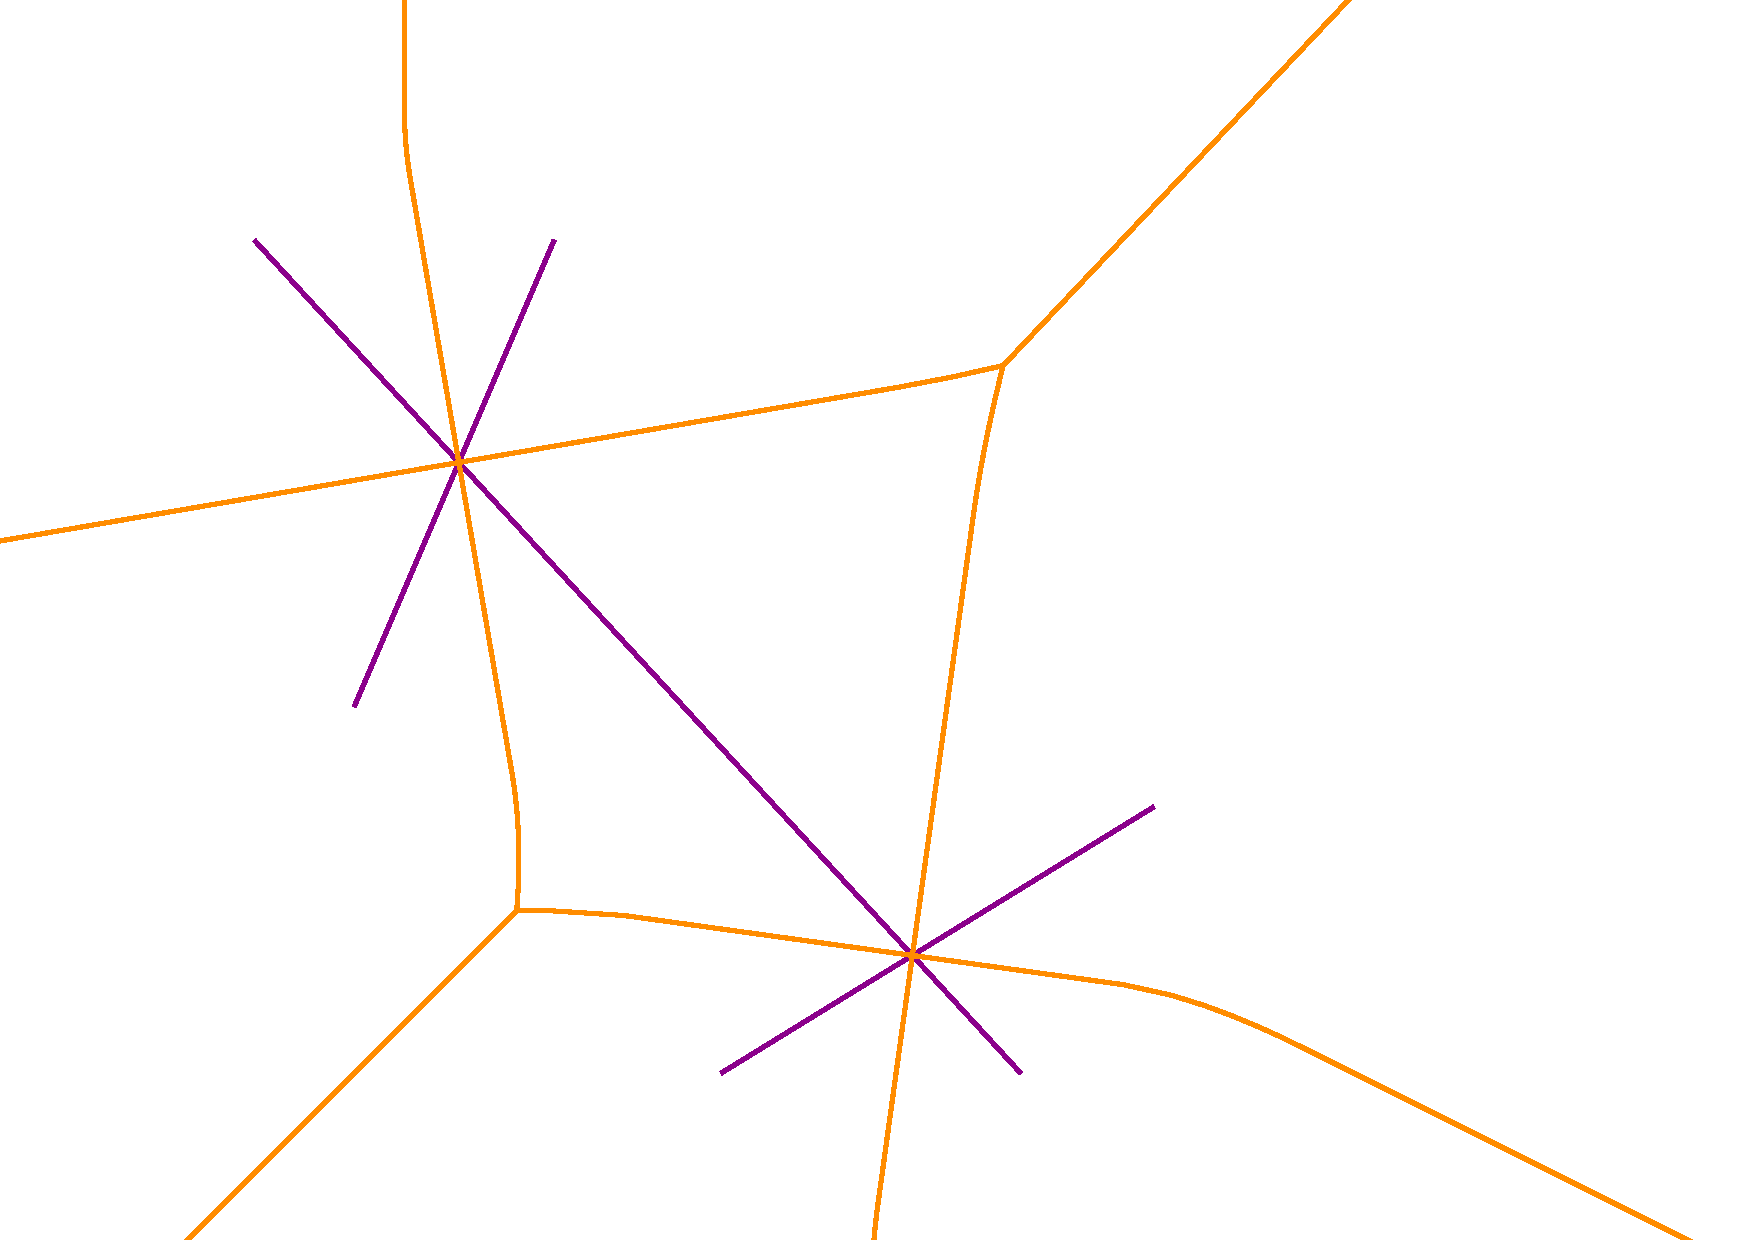
\includegraphics[width=\textwidth]{SVD_example}
        \caption{Nearest}
        \label{fig:SVD_example}
    \end{subfigure}
	\qquad
    \begin{subfigure}[b]{0.45\textwidth}
        
\includegraphics[width=\textwidth]{FSVD_example}
        \caption{Farthest}
        \label{fig:FSVD_example}
    \end{subfigure}
    \caption{Voronoi diagrams with line segments\label{fig:examples}}
	\end{figure}
	
	\subsection{CGAL and Ipelets}
	
	In this project two new functions were added to an Ipelet that already featured functions to construct Voronoi diagrams of points, Voronoi diagrams for segments, points and polygons using the \(L_{\infty}\) metric, farthest color and Hausdorff Voronoi diagrams.\par
	The two functions added are to construct, under \(L_{2}\) metric, the nearest or the farthest Voronoi diagram for line segments.\par
	For both cases the strategy used is to get the distance function of each segment as a surface, then take either the upper or the lower envelope of these surfaces (for FSVD and SVD respectively).
	
	\subsection{The envelopes strategy}
	For a single segment on the \(xy\)-plane, for every point plot on the \(z\) axis the distance of that point to the segment. This creates a 3D surface. For a point, this surface is simply a cone; for a segment, it's two haflcones originating at the endpoints of the segment and two planes originating from the inner part of the segment (figure \ref{fig:distance_function}).\par
	\begin{figure}[h]
    \centering
    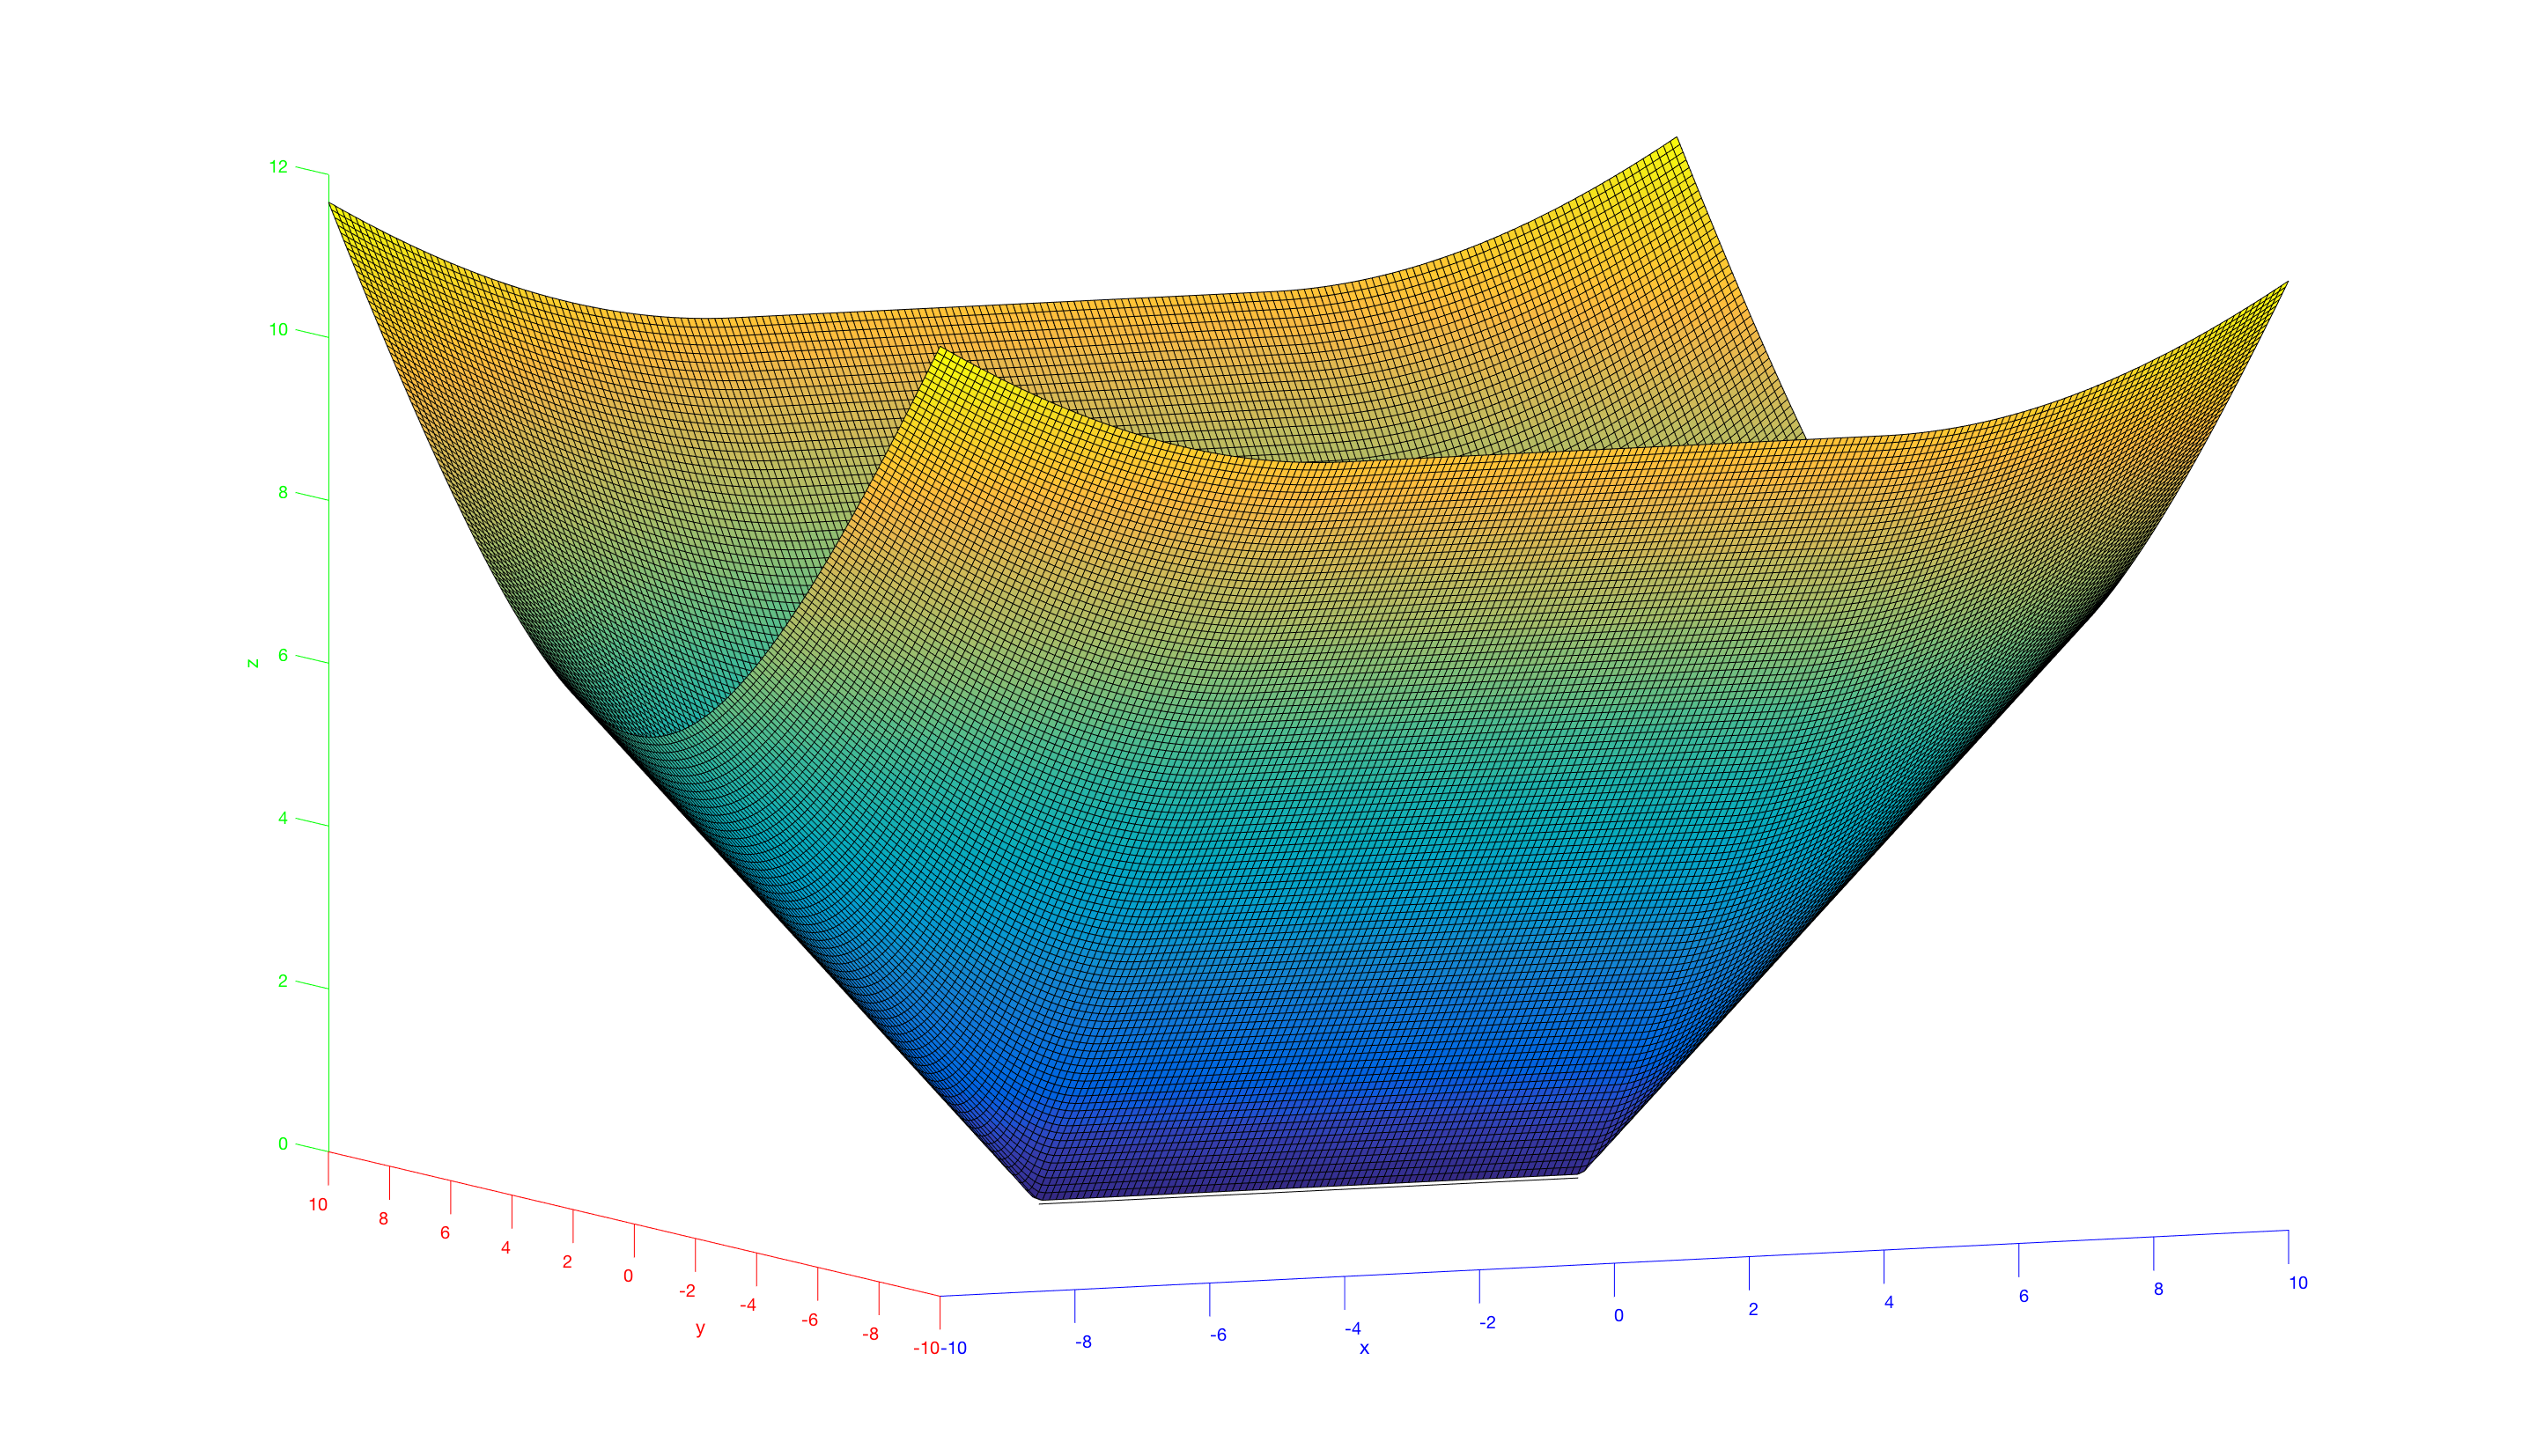
\includegraphics[width=0.8\textwidth]{distance_function}
    \caption{Distance function surface for a segment\protect\footnotemark \label{fig:distance_function}}
	\end{figure}
	\footnotetext{created using MATLAB script by Martin Suderland}
	For two distinct segments, these distance function surfaces intersect, and their intersection projected back onto the \(xy\)-plane is simply the planar euclidean bisector of the two segments.\par
	For many segments, given all their distance function surfaces, if the lower envelope is taken then the \(xy\)-projection of this envelope is the nearest Voronoi diagram, whereas the \(xy\)-projection of the upper envelope is the farthest Voronoi diagram.
	
	%____________________________________________________________

	\section{Envelope package and \cod{Envelope_diagram_2<EnvTraits>}}
	CGAL features a package to compute projections of envelopes. The methods \cod{upper_envelope_3} and \cod{lower_envelope_3} output their resulting diagram in a \cod{Envelope_diagram_2} object.
	This diagram class is parametrised by a traits class (it has to be a model of the concept \cod{EnvelopeTraits_3}) that needs to support computation of the projected boundary of a surface, the projection of the intersection of two surfaces, as well as other functions to determine the z-order of two surfaces in specific cases.
	There are already traits classes to support construction of envelopes of spheres, triangles and planes.
	
	\subsection{Traits class}
	The \cod{EnvelopeTraits_3} concept allows the surfaces to be any kind of object, as long as the required functions do their task. Because of this, for FSVD (and SVD too, they can use the same traits class) the surfaces are simply the segments themselves, since they contain all the information needed for the computations.
	In the function that requires to compute the projected intersection of two surfaces, we can in fact simply compute the planar euclidean bisector of the two segments.
	The bisector is formed, in the general case, by unbounded rays, segments and parabolic arcs (figure 5).
	
	\subsection{Arrangement traits class}
	\cod{Arr_conic_traits2}

	\subsection{Parabola class}
	A parabola class was implemented to support construction of parabolas, computation of intersection with lines and construction of arcs on the parabolas. Other predicates such as \cod{has_on} were also implemented.
	
	%____________________________________________________________

	\section{Bisector computation}
	
	\subsection{Unbounded rays}
	
	\subsection{Internal part}
	
	\subsection{Challenges and solutions}
	
	%____________________________________________________________
	
	\section{Results and future work}
	
	\subsection{Ipelet issues}
	
	\subsection{Known limitations}
	
	\subsection{Alternatives}
	
	\subsubsection{\cod{Arr_linear_segment_traits_2}}
	
	\subsubsection{Own Arrangements class}
	
\end{document}
